\subsection{Khái quát về học máy}
\subsubsection{Giới thiệu}
Học máy (\textit{Machine Learning}) là một nhánh của trí tuệ nhân tạo (\textit{AI}) tập trung vào việc tạo ra các thuật toán cho phép máy học từ dữ liệu và các thông tin có trước và tự cải thiện theo thời gian. Machine Learning cho phép máy có thể tự động học từ dữ liệu, cải thiện hiệu suất từ dữ liệu đã học được và tạo ra các dự đoán. Các thuật toán Machine Learning tạo ra các mô hình toán học hỗ trợ việc tạo ra các dự đoán hay quyết định với sự hỗ trợ từ các mẫu dữ liệu có trước hay là dữ liệu học (\textit{training data}).\cite{webpage}

Là một lĩnh vực công nghệ phát triển nhanh, học máy hiện tại được sử dụng cho rất nhiều lĩnh vực khác nhau, một số có thể kể tới là: nhận diện giọng nói, nhận diện hình ảnh hay hệ thống gợi ý sản phẩm (\textit{recommender system}).

\subsubsection{Các loại học máy}
Để có thể hiểu được cách thức mà học máy hoạt động, trước hết chúng ta cần biết về các phương pháp học máy và thuật toán, dưới đây là một số phương pháp thường dùng\cite{webpage}:
\begin{itemize}
    \item Học có giám sát (\textit{Supervised Learning}).
    \item Học không giám sát (\textit{Unsupervised Learning}).
    \item Học bán giám sát (\textit{Semi-Supervised Learning}).
    \item Học tăng cường (\textit{Reinforcement Learning}).
\end{itemize}

\subsubsection{Học có giám sát}
Các thuật toán và mô hình học có giám sát tạo ra các dự đoán dựa trên các dữ liệu đã được đánh nhãn. Mỗi mẫu dữ liệu huấn luyện đều bao gồm dữ liệu đầu vào (\textit{input}) và dữ liệu đầu ra (\textit{output}) tương ứng. Thuật toán học có giám sát phân tích dữ liệu huấn luyện và tạo ra các suy luận - hoặc có thể gọi là các suy đoán có cơ sở khi dự đoán cho các dữ liệu chưa biết trước.\cite{webpage}

Đây là hướng tiếp cận phổ biến nhất khi nói về học máy, mô hình được “giám sát” bởi chúng cần được học và cung cấp các dữ liệu đã được đánh nhãn từ trước. Dữ liệu được đánh nhãn sẽ cung cấp thông tin về các khuôn mẫu (có thể là hình ảnh, phân loại, etc) để mô hình có thể nhận diện được từ dữ liệu.\cite{webpage}

\newpage % hardcode
\begin{figure}[htb]
    \centering
    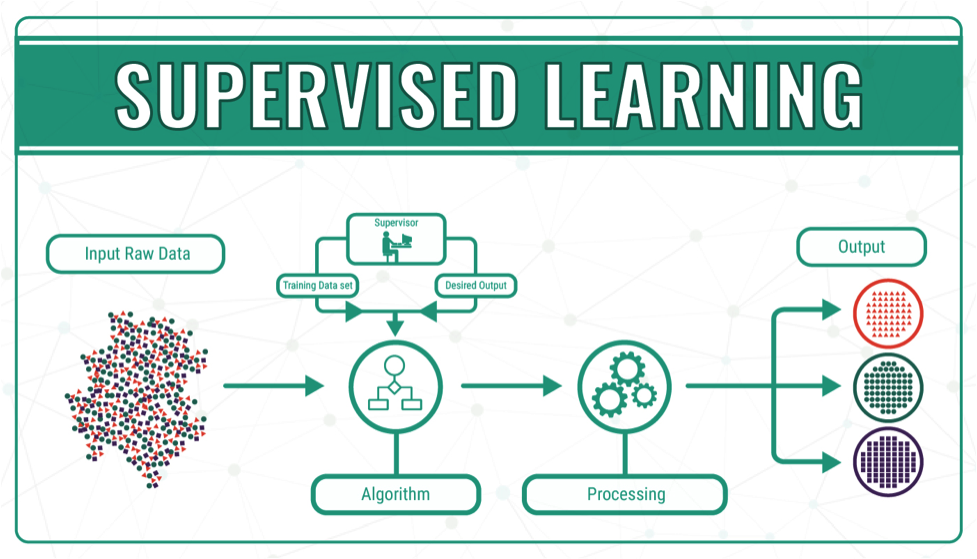
\includegraphics[width=\textwidth]{image/supervised-learning.png}
    \caption[Học có giám sát]{Học có giám sát\footnotemark}
    \label{figure:supervised-learning}
\end{figure}
\footnotetext{\url{https://dev.to/dulyaaa/lets-peek-into-machine-learning-in0}}

Và với phương pháp học có giám sát, chúng ta có hai phương pháp: phân loại (\textit{classification}) và hồi quy (\textit{regression}).
\begin{figure}[htb]
    \centering
    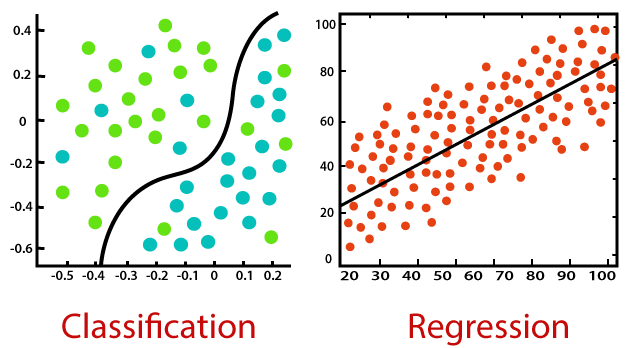
\includegraphics[width=0.7\textwidth]{image/regression-vs-classification-in-machine-learning.png}
    \caption[Phân loại và hồi quy]{Phân loại và hồi quy\footnotemark}
    \label{figure:regression-vs-classification-in-machine-learning}
\end{figure}
\footnotetext{\url{https://www.datacamp.com/blog/supervised-machine-learning}}

\begin{enumerate}
    \item Phương pháp hồi quy:
          Hồi quy tìm sự tương quan giữa biến phụ thuộc và các biến độc lập, từ đó thuật toán hồi quy có thể dự đoán các biến liên tục (\textit{continous variable}) chẳng hạn như chiều cao, cân nặng, v.v.. \cite{webpage1}

          Một số thuật toán hồi quy:
          \begin{itemize}
              \item Linear Regression
              \item Decision Tree Regression
              \item Random Forest Regression
              \item Support Vector Regression
          \end{itemize}
    \item Phương pháp phân loại:
          Phân loại là thuật toán tìm ra các hàm số có thể chia dữ liệu thành nhiều nhóm dựa trên nhiều thông số khác nhau. Khi sử dụng thuật toán phân loại, máy sẽ học trên tập dữ liệu và phân loại dữ liệu vào nhiều nhóm dựa trên những gì đã học.

          Thuật toán phân loại chuyển các dữ liệu đầu vào thành dữ liệu đầu ra rời rạc (các giá trị nhị phân như $0$ và $1$, $true$ và $false$, v.v.). Thuật toán phân loại dự đoán khả năng xảy ra của một sự kiện bằng cách đưa dữ liệu vào hàm logit.\cite{webpage1}
          \begin{itemize}
              \item Logistic Regression
              \item K-Nearest Neighbors(KNN)
              \item Naïve Bayes
              \item Decision Tree Classification
              \item Random Forest Classification
          \end{itemize}
\end{enumerate}

\subsubsection{Học không giám sát}
\begin{figure}[htb]
    \centering
    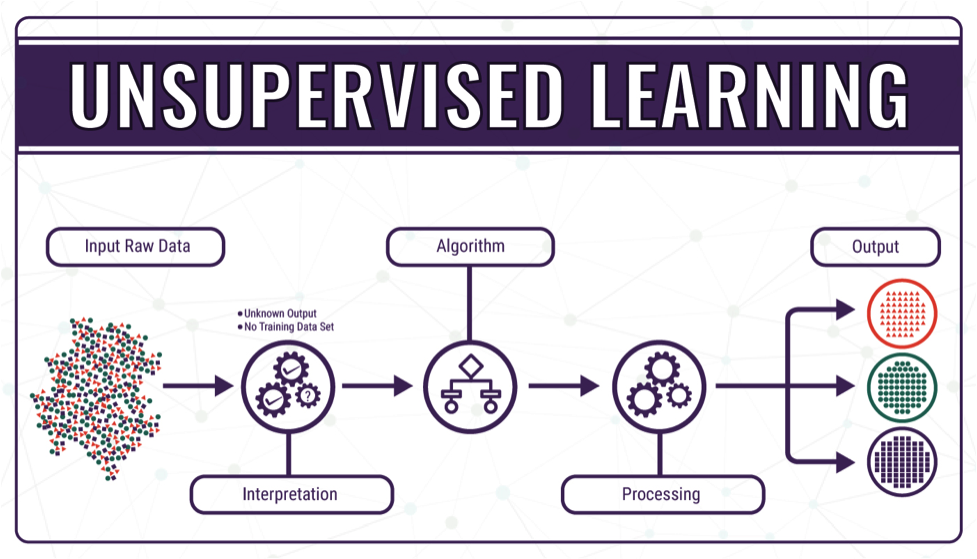
\includegraphics[width=\textwidth]{image/unsupervised-learning.png}
    \caption[Học không giám sát]{Học không giám sát\footnotemark}
    \label{figure:unsupervised-learning}
\end{figure}
\footnotetext{\url{https://dev.to/dulyaaa/lets-peek-into-machine-learning-in0}}

Các thuật toán học không giám sát khám phá các mối quan hệ trong dữ liệu không được đánh nhãn. Trong trường hợp này, mô hình được cung cấp dữ liệu nhưng không biết được dữ liệu đầu ra mong muốn, mô hình phải dự đoán dựa trên các bằng chứng gián tiếp mà không có chỉ dẫn nào. Mô hình không được huấn luyện với các ``giá trị đúng'' và phải tự tìm ra các khuôn mẫu.\cite{webpage}

Một trong những loại học không giám sát phổ biến nhất chính là gom cụm (\textit{clustering}), thực hiện gom nhóm các dữ liệu giống nhau. Phương pháp này thường được dùng trong phân tích khám phá và có thể tìm ra các khuôn mẫu hay xu hướng bị ẩn giấu.

Một số thuật toán học không giám sát:
\begin{itemize}
    \item K-Means
    \item K-Medoids
    \item Fuzzy C-Means
    \item Gaussian Mixture
\end{itemize}

\subsubsection{Học bán giám sát}
Trong học bán giám sát, dữ liệu huấn luyện sẽ được chia thành 2 phần: một tập dữ liệu nhỏ sẽ chứa các dữ liệu được đánh nhãn và tập dữ liệu lớn hơn chứa các dữ liệu không đánh nhãn.
\begin{figure}[htb]
    \centering
    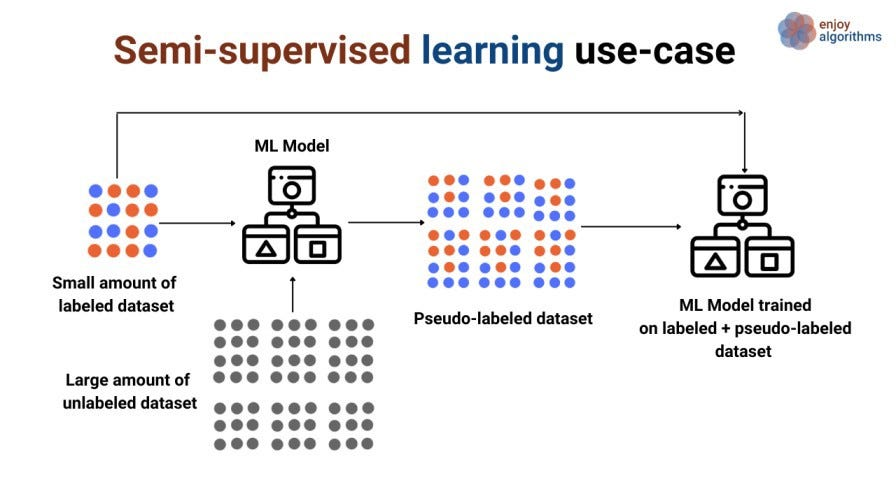
\includegraphics[width=\textwidth]{image/semi-supervised-learning.jpeg}
    \caption[Học bán giám sát]{Học bán giám sát\footnotemark}
    \label{figure:semi-supervised-learning}
\end{figure}
\footnotetext{\url{https://www.datacamp.com/blog/supervised-machine-learning}}

Trong trường hợp này, mô hình sẽ dùng dữ liệu có đánh nhãn để tạo ra các suy luận về dữ liệu chưa được đánh nhãn, cung cấp các kết quả chính xác hơn các mô hình học có giám sát thông thường.

Hướng tiếp cận này đang dần trở nên phổ biến, nhất là với những công việc sử dụng các tập dữ liệu lớn. Học bán giám sát không yêu cầu nhiều dữ liệu được đánh nhãn, dễ dàng cài đặt, và hoạt động với chi phí hiệu quả hơn các phương pháp học có giám sát, rất lí tưởng cho những công việc phải xử lý lượng lớn dữ liệu.\cite{webpage}

\subsubsection{Học tăng cường}
Học tăng cường liên quan tới việc chương trình nên hoạt động như thế nào để có được kết quả tốt nhất. Nói ngắn gọn, các mô hình học tăng cường sẽ tìm cách tốt nhất có thể để tối ưu kết quả trong một số tình huống nhất định. Quá trình này là một quá trình thử đi thử lại liên tục. Và do không có dữ liệu huấn luyện, máy phải học từ chính những lỗi sai của chúng và đưa ra lựa chọn khác để dẫn tới kết quả tối ưu.
\begin{figure}[htb]
    \centering
    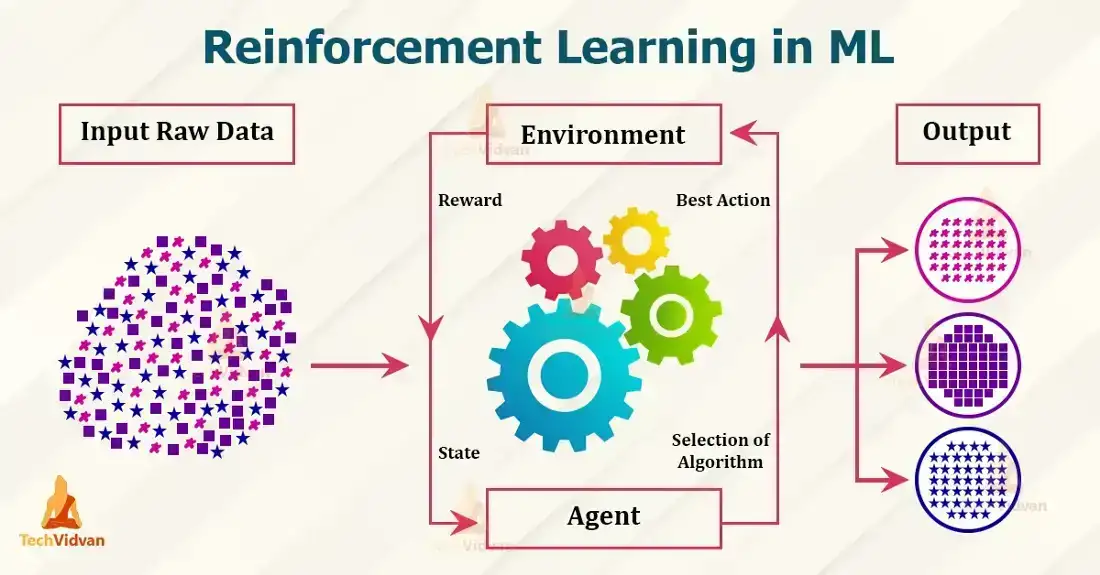
\includegraphics[width=\textwidth]{image/reinforcement-learning.jpg}
    \caption[Học tăng cường]{Học tăng cường\footnotemark}
    \label{figure:reinforcement-learning}
\end{figure}
\footnotetext{\url{https://techvidvan.com/tutorials/reinforcement-learning/}}

Phương pháp này thường được dùng trong các ngành robot và trò chơi điện tử. Các trò chơi điện tử thể hiện rõ ràng mối quan hệ giữa hành động và kết quả, và có thể đánh giá thành công thông qua điểm. Vì vậy, chúng là một cách thức thích hợp để cải thiện thuật toán học tăng cường.

\subsubsection{Cách thức hoạt động}
Hệ thống học máy xây dựng mô hình dự đoán bằng cách học các dữ liệu có sẵn từ trước và dự đoán đầu ra cho dữ liệu mới mỗi khi nhận được.

Quá trình học máy sẽ gồm 3 giai đoạn\cite{webpage2}:
\begin{enumerate}
    \item Giai đoạn 1:
          \begin{itemize}
              \item Trước khi có thể huấn luyện một mô hình học máy, chúng ta cần phải có dữ liệu. Ơ giai đoạn này, chúng ta trước hết phải thu thập dữ liệu và thực hiện tiền xử lý, nhằm đảm bảo dữ liệu không có sai sót khi đưa vào huấn luyện.
              \item Khi đã có dữ liệu, chúng ta sẽ chia dữ liệu thành nhiều phần, có thể là 3 phần (training, valid, test) hoặc 2 phần (training, test) để có thể sử dụng với mục đích tương ứng.
          \end{itemize}
    \item Giai đoạn 2:
          \begin{itemize}
              \item Sau khi đã có dữ liệu, việc tiếp theo cần làm đó chính là lựa chọn thuật toán và mô hình phù hợp. Việc lựa chọn mô hình có thể ảnh hưởng rất lơn đến kết quả cuối cùng.
              \item Sau khi đã có mô hình, chúng ta truyền dữ liệu đã chuẩn bị để mô hình có thể học và tự đánh giá.
          \end{itemize}
    \item Giai đoạn 3:
          \begin{itemize}
              \item Sau khi mô hình hoàn thiện, chúng ta tiến hành kiểm tra độ chính xác của mô hình sử dụng tập dữ liệu test đã chuẩn bị từ trước.
              \item Từ kết quả trên có thể đánh giá lại độ hiệu quả của mô hình và sử dụng mô hình khác nếu cần thiết.
          \end{itemize}
\end{enumerate}
\begin{figure}[htb]
    \centering
    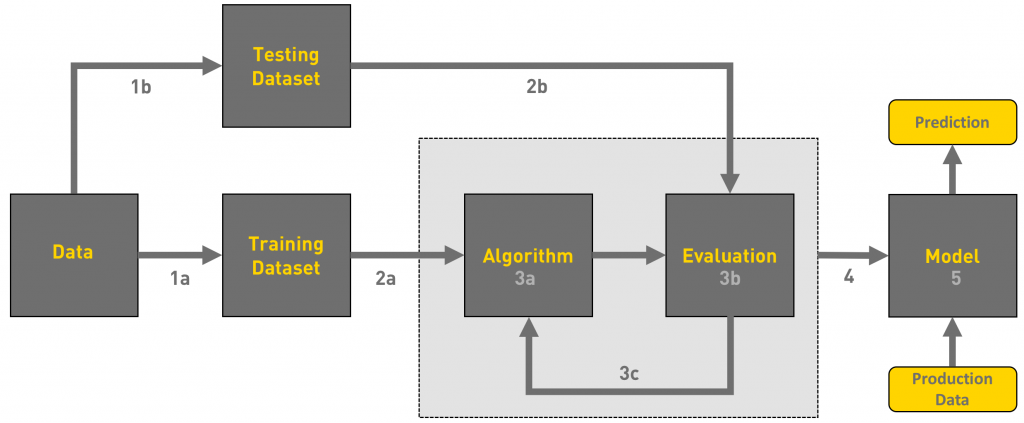
\includegraphics[width=\textwidth]{image/machine-learning-model.png}
    \caption[Cách hoạt động của mô hình học máy]{Cách hoạt động của mô hình học máy\footnotemark}
    \label{figure:machine-learning-model}
\end{figure}
\footnotetext{\url{https://www.scoutaerial.com.au/real-time-automated-shark-detection-system/}}

\subsection{Khái quát về học sâu}
\subsubsection{Giới thiệu}
Học sâu (\textit{deep learning}) có thể được xem là một nhánh của học máy. Nếu như ở học máy, các hệ thống máy sẽ học dựa trên tập dữ liệu và cải thiện nó dựa trên các thuật toán thì ở học sâu, quá trình học sẽ dựa trên các hệ thống mạng thần kinh (\textit{neural network}) - dựa trên bộ não người - để có thể bắt chước khả năng tư duy của bộ não con người.\cite{webpage10}

\subsubsection{Cơ sở hình thành}
Bộ não con người và máy tính ngay từ bản chất đã rất khác nhau, máy tính có thể dễ dàng tính toán những con số mà con người khó tính được, còn con người có thể xử lí những công việc mang tính tư duy mà máy tính không thể thực hiện. Các mạng tế bào thần kinh của con người đã tiến hóa qua hàng triệu năm và hoạt động theo cách mà con người cũng không thể hiểu hết được. Nhưng với những kiến thức đã có được về mạng thần kinh sinh học, chúng ta đã tạo ra mạng thần kinh nhân tạo dựa trên những hiểu biết đó. Tuy nhiên mạng thần kinh nhân tạo ban đầu lại không được đón nhận do sự thiếu hiệu quả so với các thuật toán truyền thống do sự hạn chế về máy móc cũng như các thuật toán truyền thống cho ra kết quả tốt với những tập dữ liệu nhỏ hơn.

Nhưng trong những năm gần đây, với sự phát triển của dữ liệu lớn (\textit{big data}) cùng với sức mạnh tính toán của máy tính đã được cải thiện, các thuật toán truyền thống không thể nào tận dụng hết được chúng, từ đó mạng thần kinh nhân tạo dần được ứng dụng nhiều hơn, cũng như sự phổ biến của học sâu.\cite{Aggarwal2022}

\subsubsection{Ưu nhược điểm}
Học sâu có một số ưu điểm vượt trội:
\begin{itemize}
    \item Kiến trúc mạng nơ-ron linh hoạt, có thể dễ dàng thay đổi để phù hợp với nhiều vấn đề khác nhau.
    \item Có khả năng giải quyết nhiều bài toán phức tạp với độ chính xác rất cao.
    \item Tính tự động hoá cao, có khả năng tự điều chỉnh và tự tối ưu.
    \item Có khả năng thực hiện tính toán song song, hiệu năng tốt, xử lý được lượng dữ liệu lớn.
\end{itemize}

Học sâu vẫn còn một số hạn chế gắn liền với nó ví dự như:
\begin{itemize}
    \item Cần có khối lượng dữ liệu rất lớn để tận dụng tối đa khả năng của học sâu.
    \item Chi phí tính toán cao vì phải xử lý nhiều mô hình phức tạp.
    \item Chưa có nền tảng lý thuyết mạnh mẽ để lựa chọn các công cụ tối ưu cho học sâu.
\end{itemize}

Tuy học sâu có hiệu năng và độ chính xác vượt trội, tuy nhiên để đạt được nó cần một lượng dữ liệu lớn và các mô hình phức tạp. Vì vậy, việc lựa chọn sử dụng học sâu hay khôn phụ thuộc nhiều vào mục tiêu của dự án, lượng dữ liệu và tài nguyên, v.v..\cite{webpage10}
